\chapter{Konzeption und Implementierung}

Das neue Konzept, das wird im diesen Kapitel erklärt, wird auf zwei großen Paketen unterteilt – Paket A und Paket B. 
Im ersten Paket wird dem Auftragsgeber User Interface (UI) aufgebaut. Das Ziel ist maximale Flexibilität des Website-Besitzers zu haben und durch einfache Tätigkeiten, bestimmten Zweck zu erreichen. Man kann editieren, ändern und Text stilisieren. Umbraco verfügt mit sogenannte „Grid“. Es dient dafür, dass man das Design der Seite manipulieren und auch die schon besprochenen Möglichkeiten ausnutzen kann. 
Es werden auch eigene Macros benutzt, in den ein Quell-Code der SHOP – Komponenten hingeschrieben wird. Somit kann der Auftragsgeber Macros in beliebigen Teilen der Seiten hinstellen. Umbraco – Forms werden benutzt als Formulare, damit man selber einordnen kann.
Beide Paketen werden als Startknoten aus einer Umbraco-Instanz heraus verwaltet. 
Paket B ist als Kern der Seite dargestellt. Das ist eigentlich das Online-Bestellsystem. Hier ist es wichtig, dass eine unkomplizierte, bedienbare, reibungslose und flexibel Umgebung aufgebaut wird. Das System besteht aus drei Hauptkerne: 
\begin{itemize}	
	\item Bestellsystem
	\subitem Kundenverwaltung (Anmeldung, Kundenbereich, Kommunikation)
	\subitem Artikelverwaltung
	\subitem Auftragsverwaltung
	\item E-Mail-Verwaltung
	\subitem E-Mail-Vorlagen anlegen, editieren, löschen
	\item Umsatzerfassung
	\subitem Umsatzübersicht nach Monat und Jahr
\end{itemize}

\section{Aufbau vom Umbraco}
Wie oben schon erklärt wurde, ist Umbraco ein Content Management System, das flexibel und Benutzerfreundlich ist. Damit man bessere Verständnis hat, worum es geht, wird es im nachträglichen Unterkapitel erläutern. 

User Interface von Umbraco ist auf drei Teilen verteilt. Erste Teil ist Hauptfunktion bzw. Setcion bezeichnet. Da befinden sich die Hauptoptionen: Content, Media. Settings, Developer, Users, Members, Forms.
Damit einen klaren Unterschied zwischen „Member“ und „User“ gemacht wird, werden die beiden Begriffe erklärt. „User“ ist jemand, der Zugriff zu „Umbraco-Backoffice“ hat und dort hat bestimmte Rechte. 

Ein Member wird von Umbraco für die Registrierung und Authentifizierung eines externen Besuchers benutzt. Das sind Leute, die nur Front-End benutzen dürfen. 
Man kann auch „Custom Setcion“ erstellen, womit wir uns im weiteren Kapitel beschäftigen. 

Nächste Teil ist Unternavigation oder auch Tree genannt. Alle Unteroptionen stehen da. Jede Hauptfunktion hat ihre eigenen Unteroptionen.
Es wird zum jeweiligen Setcions zugehörige Funktionalität der Unteroptionen (Trees) durchgehen.

\begin{itemize}	
	\item\textbf{Trees vom Content-Section:} In diesem Tree befinden sich alle Seiten, die im Website Front-End er-schienen werden können. Da steht auch Recycle Bin, oder auch Papier-korb genannt. So kann man die gelöschte Seite zurücksetzen. 
	\item\textbf{Trees von der Media-Section:} Hier können alle Videos und Bilder stehen
	\item\textbf{Trees vom Settings-Section:}Mithilfe von (PartialView), HTML, CSS, JavaScript, Dokument- und Medientypen, das Erstellen und das Einsetzen von Templates und Spracheinstellungen werden die Webseiten einfach und schnell eingerichtet.
	\item\textbf{Trees vom Developer-Section:} Hier stehen zur Verfügung Trees, die es den Entwickler ermöglichen bereits erstellte Seiten zu entwickeln. Das wird durch Data Typ, Macros, Packages, Relation Types, XSLT Files und Partial View Macro Files ermöglicht.
	\item\textbf{Trees vom User:}In diesem Bereich stehen die Benutzer, die mit bestimmtem Rechten vom Umbraco die Front-End der Webseite benutzen dürfen. Zu einem be-stimmten User können verschiedene Rechte abgegeben werden. 
	\item\textbf{Trees vom Member-Section:} Hier sind Benutzer, die sich in der fertigen Webseite registriert haben.
	\item\textbf{Trees vom Forms-Section: } Hier kann man leicht verschiedene Arten von Formularen erstellen.		
\end{itemize}

Der dritte Teil vom Umbraco-Backoffice ist der Editierbereich. Dort werden alle Eigenschaften von jeweiligen Tree-Optionen dargestellt.

Im Abbildung \ref{fig:Umbraco Backoffice} kann man sehen, wie Umbraco-Backoffice aussieht.
\begin{figure}[h]
	\centering
	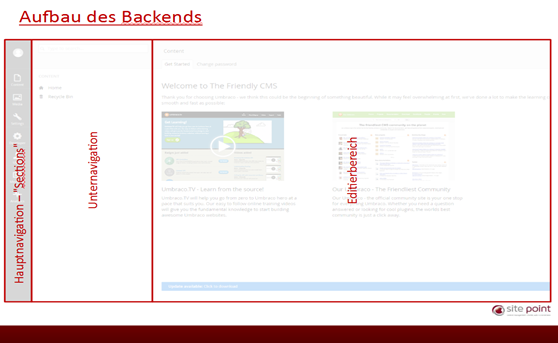
\includegraphics[width=1\linewidth]{Graphics/UmbracoBackend.png}
	\caption[Umbraco Backoffice]{Übersicht vom Umbraco-Backoffice}
	\label{fig:Umbraco Backoffice}
\end{figure}

\pagebreak
\section{Kundenverwaltung}
Die Kundenverwaltung fasst den ganzen Bereich um, der sich um die Kunden bezieht. Mehr wird in nächsten Unterkapitel erfahren.

\subsection{Kundenerfassung}
1. Das angestrebte Ziel ist, dass der Kunde sich registrieren kann. Die Registrierung muss gesichert und individuell sein. Damit die Registrierung zuverlässig ist, muss nach den folgenden Regeln gehalten werden: Vertraulichkeit, Integrität, Verfügbarkeit und Authentizität.
Ein \ac{PIN} lässt sich in E-Mail des Kunde zusenden. So wird sichergestellt, dass die Kunde eine gültige E-Mail hat. Nach der Registrierung wird überprüft, ob die E-Mail schon existiert. Wenn ja, das Prozess wird storniert und eine Nachricht erscheint, in der geschrieben ist, dass der Kunde diese E-Mail schon verwendet hat. 
Der Auftragsgeber entscheidet, ob der sich registrierten Kunde bestellen darf    oder nicht. Danach kann der Benutzer sich mit dem PIN und die E-Mail anmelden. 
Die Kundenverfassung wird durch Member \ac{API} von Umbraco realisiert. 
Wie schon erläutert wurde, ist Umbraco auf ASP.NET basiert. Damit kann man vom CMS unterschiedliche „Services“ benutzen. Ein davon ist „MemberService“. Das ist direkte Kanal zu dem MemberAPI. Es ist in den „Services property“ von dem „SurfaceController“ zu Verfügung gestellt. 
Die Registrierung wird via ASP.Net Code und Media API programmatisch erstellt. Das ist eine komplexe Methode, in der es eine vielfältige Datei benötigt wird (SurfaceController, Model, PartialView und Source Datei, wo Front-End Sourcecode steht). Die benötige Information, die wir zu der Registrierung brauchen, wird im „Model“- Datei geschrieben. 
In der Datei „Model“ stehen „Model Properties“. Das sind Parametern, mit denen man arbeitet. Einfach erklärt, über das Model werden die Properties von „Partial-View“ zu dem „SurfaceController“ übertragen.
„SurfaceController“ ist der „Autobahn“ zu der Umbraco-Datei. Das ist ein MVC (Model View Controller), das mit dem Umbraco interagiert wird. Es wird von der Bibliothek Umbraco.Web.Mvc.SurfaceController geerbt. 
Über „PartialView“ werden die Verbindungen zwischen Kontakt Formular und „Model Properties“ geschehen. Das ist eigentlich eine Teilansicht, die von Umbraco Front-End benutzt wird. Dort ist Umbraco User Interface (UI). 
Folgende Abbildung \ref{fig: neues Konzept: Registrierung} ergibt bessere Verständnis wie die obengenannten Begriffe zu einander stehen.

\begin{figure}[h]
	\centering
	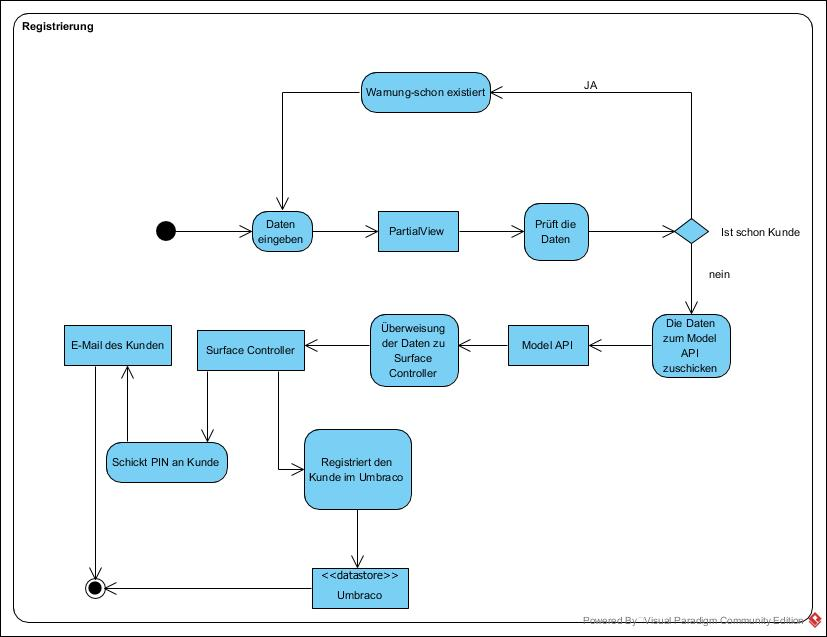
\includegraphics[width=\paperwidth,angle=90]{Graphics/Registrierung.JPG}
	\caption[neues Konzept: Registrierung]{Neues Konzept zum Registrieren}
	\label{fig: neues Konzept: Registrierung}
\end{figure}

Diese Möglichkeit vom Umbraco erlaubt uns sich sehr leicht und bequem in dem Server anzumelden.
In Anhang 6 kann man sich übersichtlicher genau anschauen, was im Back-End passiert ist.

\subsection{Kundeansicht}
Für Erleichterung des Kunde stehen auf einer Seite alle Möglichkeiten, die der Kunde hat: 

\begin{itemize}	
	\item Neue Bestellungen abgeben, aktuelle und vorherige Bestellungen ansehen
	\item Neue Nachricht schreiben und alte Nachrichten ansehen.
	\item Wichtige Information zu beachten
	\item Individuelle Information vom Auftraggeber.
\end{itemize}
Nach der Registrierung wird der Kunde eine neue Seite sehen. Dort kann er die obengenannten Optionen verwalten. 
Wenn der Kunde neue Bestellung tätigen will, wird ein neues Fenster geöffnet, in dem er erwünschten Artikeln wählen und bestellen kann. Die gewählten Produkte werden in den Datenbanken gespeichert. Von dort werden sie als vergangene Bestellungen verwendet. Das selben Prinzip steht auch für die Kommunikation zwischen den Auftragsgeber und den Kunden. Wenn eine Nachricht ge-schrieben wird, wird sie in den anderen Datenbanken gespeichert. 
Vom Umbraco wird die Information direkt zu den Kunden gesendet. 
Der Auftragsgeber, so wie der Kunde, können von der Datenbank die Bestellungen und die Nachfragen ansehen.

